
\subsection{Live Bus Arrivals API Stream}
\par The Live Bus Arrivals API Stream provides the predicted time until a bus is expected to arrive at a stop. These predictions are available for the next 30 minutes at any point in time. For example, at 9am, the stream will provide predicted bus arrivals up to 9.30am on the same day. This data is refreshed every 30 seconds \cite{live_bus_api_documentation}.

\par In order to collect bus arrival data for analysis, we supplied the following selected parameters to the API. These parameters specify the fields returned by the API. We then stored the data received to a MySQL database continuously.

\subsubsection{Parameters supplied}
\begin{itemize}
	\item \textit{StopID} This is the alphanumeric identifier of a bus stop.
  \item \textit{LineName} This is the route number that is displayed on the front of the bus on any publicity advertising the route.
	\item \textit{VehicleID} The unique identifier of the vehicle.
  \item \textit{DirectionID} This identifies the direction of the trip (either outbound or inbound) that the vehicle is on.
  \item \textit{TripID} The identifer of the specific trip that the prediction is for.
  \item \textit{EstimatedTime} This is the predicted time of arrival for the vehicle at a specific stop.
  \item \textit{ExpireTime} This is the time at which the corresponding prediction is no longer valid and should stop being displayed.
\end{itemize}

\par Each data entry contains an estimated arrival time for each bus journey at a given bus stop. This estimated arrival time is stored in the database via an UPDATE statement, which ensures that only the latest estimated arrival times per journey per bus stop are stored. This has been achieved through running a daemon process written in python on a virtual host. Figure \ref{fig:arrivals_schema} shows the schema for arrivals table. See Figure \ref{fig:arrivals_view} for sample data stored.

\begin{figure}
\centering
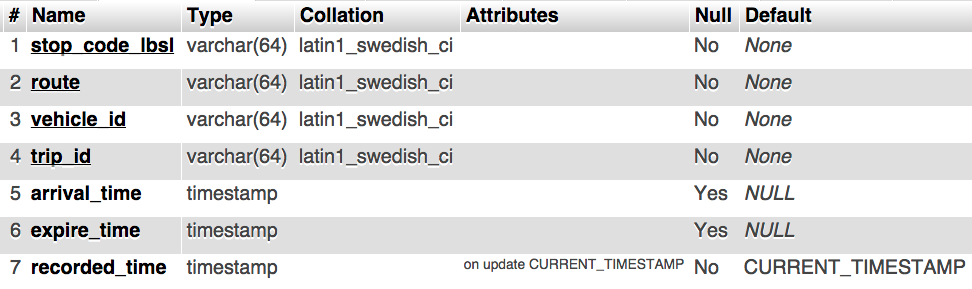
\includegraphics[width=0.9\textwidth]{figures/arrivals_schema.png}
\caption{\label{fig:arrivals_schema} Arrivals table schema }
\end{figure}

\begin{figure}
\centering
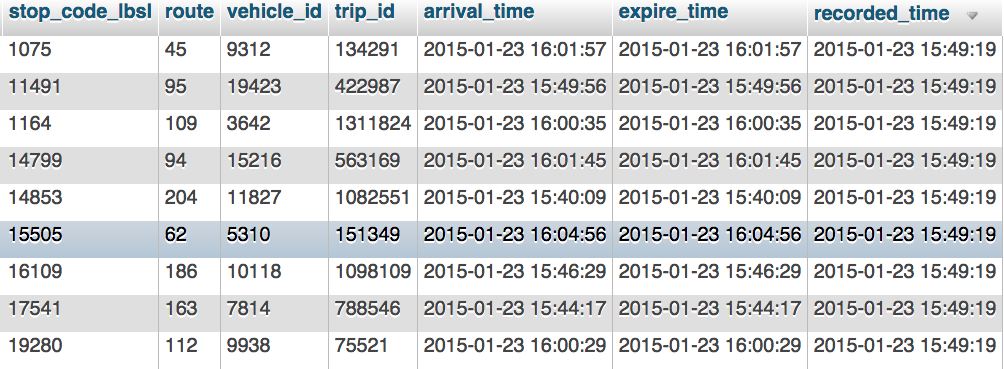
\includegraphics[width=0.9\textwidth]{figures/arrivals_view.png}
\caption{\label{fig:arrivals_view} Data stored in arrivals table}
\end{figure}


\subsubsection{Assumption}
We assume that the actual bus arrival time is the midpoint between the last estimated arrival time, and the system time when the clear signal (ExpireTime = 0) is received.

